\chapter{Comunidades virtuales}
\label{comunidades-virtuales}

Se denomina \textbf{comunidades virtuales} a determinados grupos de sujetos (individuos, colectivos e instituciones) que concentran sus esfuerzos en el ordenamiento de datos procesados en Internet, a partir de servicios en línea. En otras palabras, son grupos de individuos e instituciones organizados cibernéticamente en torno a un margen de intereses específicos, cuyas interacciones, vínculos, relaciones y comunicaciones se dan a través de la red.

Las comunidades virtuales pueden ser muy diversas y específicas, involucrando personas de procedencias alejadas geográfica y culturalmente, ordenadas en torno a un tema común de su pasión o interés, y un \textbf{espacio virtual} que puede estar determinado por una página web o un servicio on-line.

El término \href{https://es.wikipedia.org/wiki/Comunidad_virtual}{comunidad virtual} se empleó por primera vez en 1994, en el libro La comunidad virtual: \href{https://www.casadellibro.com/libro-la-comunidad-virtual-una-sociedad-sin-fronteras/9788474325621/542034}{una sociedad sin fronteras} de \href{https://es.wikipedia.org/wiki/Howard_Rheingold}{Howard Rheinhold}. Sin embargo, las primeras comunidades virtuales ya existían desde los años 70 del siglo XX, particularmente en torno al intercambio de datos especializado en ámbitos militar, científico y académico, gracias a los mecanismos de comunicación de la entonces rudimentaria Internet, como sistemas de boletín o tablones de anuncios.

Actualmente las comunidades virtuales son un fenómeno masivo en línea y muy vinculado a la explosión de las redes sociales, capaces de interconectar este tipo de organizaciones virtuales o de crear otras propias, en torno a ejes comunicativos masivos y distintos tiempos y modos de interacción.

En principio, las comunidades virtuales tienen como propósito el \textbf{intercambio de información} especializada en torno a un tema o un eje de temas que puede ser cualquiera, desde ciencia y tecnología, creación literaria, fanatismo deportivo o cinematográfico, etc. Quienes colaboran en ellas son a la vez consumidores, productores y/o replicadores de la información disponible al respecto.

Por otro lado, son una herramienta útil para los ámbitos corporativos, permitiendo una organización interna de las comunicaciones, tanto como un contacto más estrecho y directo con los consumidores, organizando una comunidad en torno al producto o a la marca (\href{https://rockcontent.com/es/blog/branding/}{branding} o fidelización). Igualmente opera como un espacio de socialización e intercambio de diversa naturaleza entre personas de todo tipo, en el marco de las redes sociales y la \href{https://comunidad.iebschool.com/culturaempresarial/2016/11/21/la-cultura-2-0/#:~:text=La\%20Cultura\%202.0\%20o\%20digital,sino\%20de\%20valores\%20y\%20de}{cultura 2.0}.

Las comunidades virtuales suelen caracterizarse de la siguiente manera:
\begin{itemize}
    \item Involucran individuos de distinta procedencia, que pueden provenir de geografías distantes, grupos sociales diversos, etc.
    \item Organizan a sus miembros en torno a un tema específico o un interés específico, ya sea el debate en torno a ciertos tópicos, la creación literaria conjunta, los videojuegos, la oportunidad de citas románticas, etc.
    \item No posee un anclaje físico en el mundo real, sino en un servicio o página Web disponible de manera digital.
    \item Imprime un sentido de pertenencia en sus miembros tan fuerte como las comunidades tradicionales, ya sea que se preste o no para el intercambio físico y presencial.
\end{itemize}

\section{Redes sociales}

La llegada de Internet, hace ya algunos años, generó un antes y un después en las diferentes civilizaciones, sobre todo porque abrió paso a una nueva manera de comunicación entre usuarios que no necesariamente necesitaban estar dentro de la misma habitación. Por ejemplo, con el correo electrónico, las páginas web o los foros. La interacción entre personas empezó a ganar, poco a poco, más y más fuerza, eliminando -entre otras cosas- gran cantidad de fronteras culturales o idiomáticas. Y, como no podía ser de otra manera, dentro de este escenario surgieron, también, las redes sociales, cuyo éxito radica fundamentalmente en la posibilidad que ofrecen a los usuarios de comunicarse con otros, de manera totalmente inmediata, a través de espacios virtuales, sin importar en qué lugar del planeta se encuentren.

Las comunidades virtuales y las redes sociales son dos conceptos diferentes. Se habla mucho, en el mundo del marketing, de comunidades virtuales y redes sociales y, muchas veces, se hace de forma indistinta, pero existen algunas diferencias. Para entender la diferencia entre comunidades virtuales y redes sociales,  es necesario entender en qué se centra cada una de ellas:
\begin{itemize}
    \item Jerarquización. En las redes sociales no hay jerarquía. Sin embargo, en las comunidades virtuales siempre hay una jerarquía.
    \item Información. Aunque todas están encaminadas a permitir el flujo de información, las comunidades basan su existencia en ese hecho. Se podría tener una red social como mero repositorio de contactos, pero no se podría tener una comunidad en la que no hubiera acción.
    \item Objetivo. Las redes sociales basan su objetivo en el ocio/networking, mientras que las comunidades tienen un objetivo más específico.
    \item Marketing. Desde el punto de vista del marketing las redes sociales generan nuevas tendencias y crean eventos. Las comunidades ayudan a segmentar a los usuarios con mayor precisión.
\end{itemize}

\section{Historia de las redes sociales}

Para empezar es necesario recordar el nacimiento de Internet, allá por 1947, cuando la Guerra Fría daba sus primeros pasos, enfrentando a ciudadanos de extremo a extremo del mundo; unos occidentales y capitalistas (liderados por Estados Unidos), y otros orientales y comunistas (liderados por, entonces, la Unión Soviética). Una auténtica batalla por el poder que motivó numerosos avances tecnológicos. Entre ellos, EEUU creó la Advanced Research Projects Agency (ARPA), la que -una década más tarde- asentó los pilares de lo que sería conocido como Internet, ya que su red ARPANET permitía el intercambio de información entre instituciones.

Gracias a esto, con el paso del tiempo, usuarios de diferentes partes del mundo empezaron a estar en contacto gracias a los correos electrónicos (siendo el primero enviado en 1971) o al Proyecto Gutenberg (Biblioteca Online gratis), en 1971. Unos años más tarde, en 1991, la red de Internet global se hizo pública, con el World Wide Web (lo que, comúnmente se conoce como «www»), y así surgió Internet.

\subsection{Primera red social: SixDegrees}

A pesar de todos estos avances, no existía aún ningún elemento, herramienta o aplicación que permitiese a los usuarios socializar entre ellos, más allá del intercambio de emails o los programas de chat online, como IRC. Esto cambió en 1997, cuando se creó SixDegrees, la que puede considerarse como la primera red social del mundo; una red que permitía localizar a otros miembros de la red y crear listas de amigos, y que se basaba en la teoría de los seis grados de separación, que afirma que es posible conectar con cualquier otra persona del mundo en tan solo 6 pasos.

\begin{figure}[ht!]
    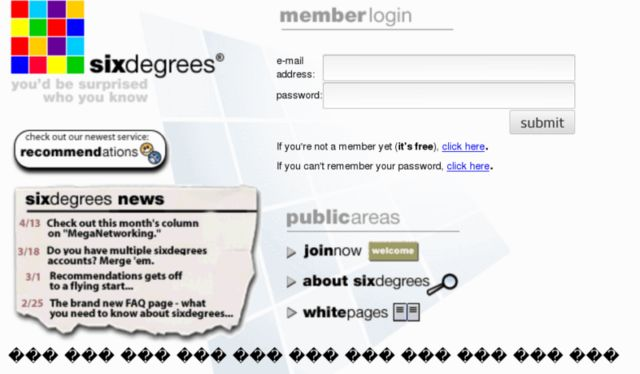
\includegraphics[width=\textwidth]{sixdegrees.jpg}
    \caption{Six degrees}
    \label{sixdegrees}
\end{figure}

Tal y como explicó Andrew Weinreich, su creador, el día de su lanzamiento:

«El desafío es construir una comunidad, el desafío es encender una llama. Este es un servicio que pueden usar para hacer sus vidas más eficientes. Pero, al igual que comprar una libreta de direcciones, si no le añades nombres es inútil».

La aplicación era básicamente una red que unía a conocidos con «conocidos de conocidos». Sin lugar a dudas, puede considerarse una red fallida en términos comerciales, pero es innegable que cimentó las bases de lo que hoy se conoce como redes sociales. La aplicación cerró en 2001.

\subsection{La llegada de Friendster, MySpace y LinkedIn}

En 2001, SixDegrees desapareció, pero fueron solamente necesarios unos meses más para que los entonces afortunados usuarios digitales pudieran empezar a disfrutar de nuevas redes sociales, como Friendster, que se creó en 2002 como una red social para amantes de los videojuegos.

\begin{figure}[ht!]
    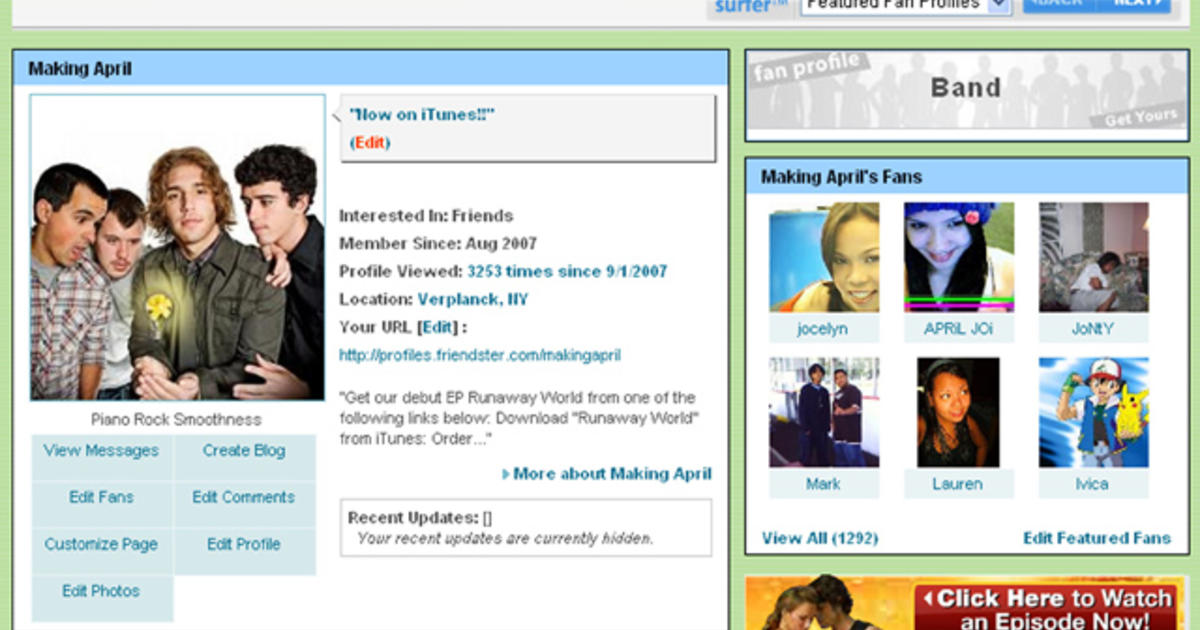
\includegraphics[width=\textwidth]{friendster.jpg}
    \caption{Friendster}
    \label{friendster}
\end{figure}

Por otro lado, MySpace y LinkedIn aparecieron en 2003, considerándose redes mucho más profesionales y orientadas a empresas. Se trata de redes sociales antiguas, muchas de las cuales desaparecieron, aunque no todas. Sobre todo LinkedIn, cuyo impacto en el mundo empresarial fue inmediato llegando, en 2008, a disponer de más de 25 millones de usuarios registrados, extendiéndose a empresas de 150 sectores diferentes. Hoy en día, la misma cuenta con más de 600 millones de usuarios registrados.

\subsection{Nacimiento de Facebook}

En 2004 un joven universitario procedente de la Universidad de Harvard colocó la guinda del pastel, y creó la red social más importante, en la actualidad, del mundo: Facebook. Aquel joven estudiante era Mark Zuckerberg.

La historia de Zuckerberg y de cómo creó Facebook es apasionante: Zuckerberg creó, en aquel entonces, un portal llamado Facemash cuya finalidad no era otra que la de poder conectar a los estudiantes de Harvard entre ellos, para disponer -así- de un lugar virtual donde compartir opiniones acerca de quiénes eran las personas más y menos atractivas de la universidad; algo que llegó a la dirección de la misma, generando la expulsión del estudiante.

\begin{figure}[ht!]
    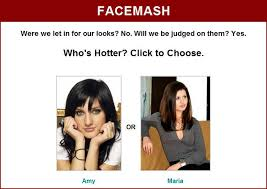
\includegraphics[width=\textwidth]{facemash.jpeg}
    \caption{Facemash}
    \label{facemash}
\end{figure}

No obstante, su habilidad informática se dejó ver tan claramente con aquella aplicación, que poco duró en evolucionar y crecer a lo que es hoy en día.

\subsection{Nacimiento de YouTube}

Solamente un año más tarde, en 2005, surgió una nueva revolución, que hoy en día se mantiene como una de las redes sociales más importantes: YouTube. Una red creada por Chad Hurley, Steve Chen y Jawn Karim en San Bruno, California. Según cuenta la leyenda, la idea de YouTube surgió ante las dificultades que los 3 jóvenes encontraron para compartir una serie de vídeos con sus amigos, mientras se encontraban en una fiesta en San Francisco.

El 23 de abril de 2005 fue subido el primer vídeo a la red: Me at the Zoo

\begin{figure}[ht!]
    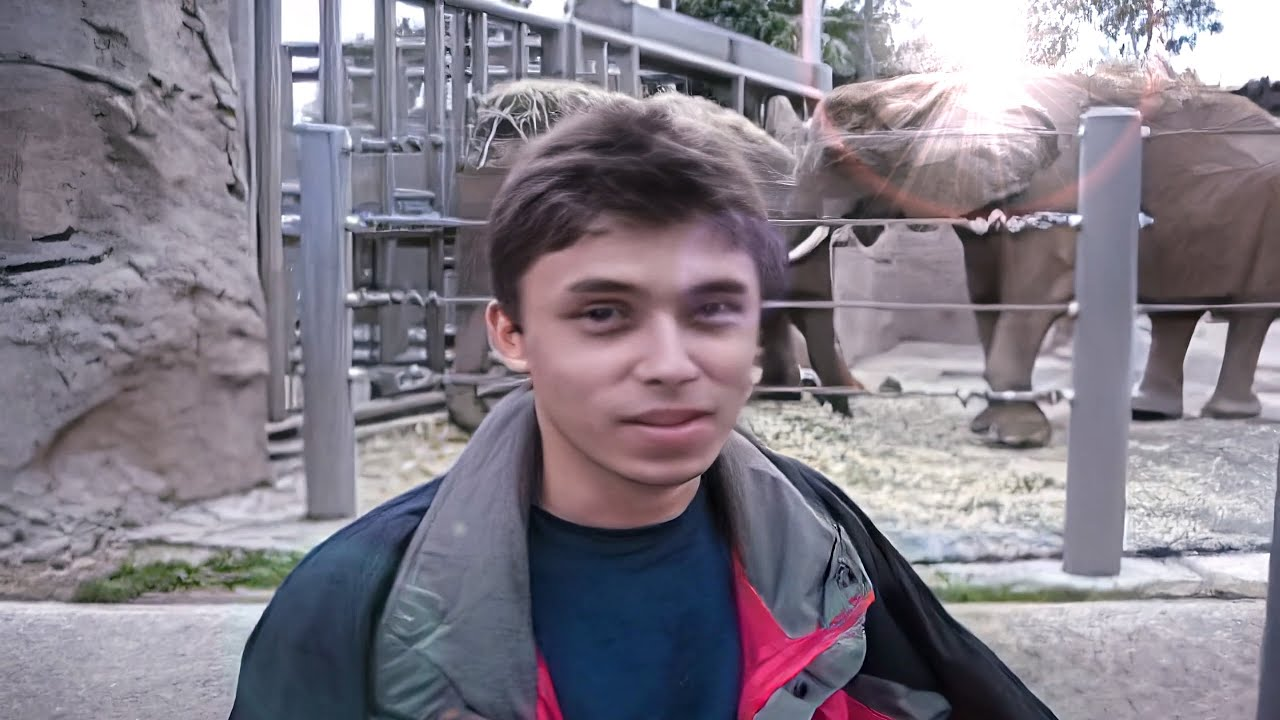
\includegraphics[width=\textwidth]{zoo.jpg}
    \caption{Me at the zoo}
    \label{zoo}
\end{figure}

El bombazo de esta red fue tal, que rápidamente usuarios de todo el mundo empezaron a subir vídeos de todo tipo a la red, perdiéndose ligeramente la idea original de la misma. Pero, sin embargo, el tráfico se disparó aún más cuando los usuarios empezaron a colocar enlaces de YouTube en sus páginas de MySpace.

\subsection{Nacimiento de Twitter}

En 2006 surgió, en San Francisco y de la mano de Jack Dorsey, Noah Glass, Biz Stone y Evan Williams, la red social de \textbf{microblogging}: Twitter, que inicialmente se llamó twttr, para evolucionar después al nombre actual. Fue, sin duda, la revolución de la comunicación. La «corta ráfaga de información intrascendente«, o el trino de un pájaro, que, en inglés, se dice \textbf{tweet}.

Hoy en día, el impacto de esta red es tal que incluso medios de comunicación, como televisiones, radios y medios de noticias digitales, dedican espacios enteros a hablar del impacto que algún tweet, tendencia o mención especial ha tenido sobre alguna noticia del momento. Y, a pesar de que cuenta con algún que otro detractor, lo cierto es que muchos achacan su éxito a la sencillez de su uso; el mismo uso que en su origen: el de un número de caracteres limitados que permiten a sus usuarios comunicarse entre ellos.

\begin{figure}[ht!]
    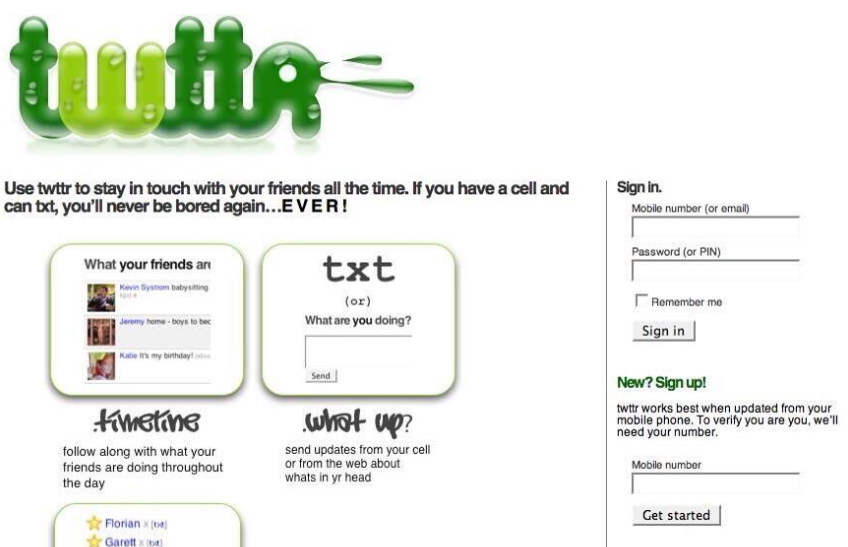
\includegraphics[width=\textwidth]{twitter-first.png}
    \caption{Twttr}
    \label{twttr}
\end{figure}

\subsection{Nacimiento de WhatsApp}

La que hoy en día se puede considerar como la \textbf{app de mensajería instantánea} más famosa surgió en 2009, y fue creada por el ucraniano Jan Koum. La misma se creó, originalmente, con la utilidad de ser una agenda inteligente -de ahí que se vincule con la agenda de contactos de nuestro terminal móvil-, permitiendo al usuario ver qué estaba haciendo cada persona en cada momento, con la finalidad de saber si podía iniciar o no una conversación con él. De ahí, su nombre: WhatsApp («¿Qué hay?», «¿Qué pasa?»)

Hoy en día, supera los 2.000 millones de usuarios, encontrándose por encima de aplicaciones como \href{https://www.facebook.com/messenger}{Facebook Messenger} o \href{https://play.google.com/store/apps/details?id=org.telegram.messenger&hl=es&gl=US}{Telegram}. En 2014, fue comprada por Mark Zuckerberg -el creador de Facebook- por, nada más y nada menos, que 19.000 millones de dólares.

\subsection{Nacimiento de Instagram}

En 2010, Instagram llegó al mercado, posicionándose rápidamente como la red social más fotográfica por excelencia, con un éxito superior a otras opciones como Flickr. Instagram fue creada por Kevin Systrom y Mike Krieger, y la particularidad con la que contó en sus inicios (que hoy en día se mantiene) es que trataba sus imágenes y fotografías de una forma cuadrada, en honor a la Kodak Instamatic así como a las cámaras Polaroid, contrastando con la relación de aspecto más vertical con la que hoy en día cuentan la mayoría de las cámaras de los terminales móviles. Además, fue la red pionera, junto con Twitter, en la popularización de los \textbf{hashtags}, allá por enero de 2011, buscando facilitar a los usuarios el descubrir las fotografías que los demás usuarios compartían sobre un mismo tema, y que no podían llegar a visualizarse de otra manera.

Instagram alcanzó una gran popularidad en sus primeros meses de vida, llegando a tener más de 100 millones de usuarios activos en abril de 2012 (solo dos años después), y más de 300 en 2014. A día de hoy, aún sigue creciendo más y más, sobre todo debido a que se trata de una red social enfocada a las nuevas generaciones, que tanto pecan de estar 24/7 mostrando a sus contactos qué están haciendo, en forma de fotografías colocadas en su \textbf{feed} o en sus \textbf{stories} (un formato que se define por hacer público contenido que desaparece a las 24 horas, en el que \href{https://www.snapchat.com}{Snapchat} fue pionero, y, tiempo más tarde, llegó a Instagram y a Facebook). Precisamente, esta medida, la de lanzar sus propias stories, fue clave en el destino de Snapchat, la red social que en su momento estuvo en boca de todos como la de mayor auge a nivel mundial, y que acabó languideciendo en gran parte del mundo, ensombrecida por el poder de Instagram.

\subsection{Nacimiento de Pinterest y Google Plus}

A partir de entonces, cada año fueron surgiendo nuevas redes sociales con diferentes funcionalidades o destinadas a distintos grupos. Pinterest, por ejemplo, una red social que colecciona imágenes -sobre todo, de inspiración- que permite a los usuarios almacenarlas en tableros y dotarlas de «pines», fue creada en 2010 y, a los 9 meses de su lanzamiento, ya disponía de 10.000 usuarios. 

Por su parte Google+ fue el gran intento fallido del gigante online. Surgió en 2011, fue una red social propiedad de Google, que llegó a alcanzar los 10 millones de usuarios tan sólo dos semanas después de su lanzamiento. Tras 3 semanas de funcionamiento, ya rondaba los 20 millones. Una red que realizó grandes esfuerzos por desafiar a otras como Facebook, LinkedIn, MySpace, Vimeo o Tumblr, pero que cerró sus puertas en abril de este 2019.

\subsection{Nuevas redes sociales}

Con el paso del tiempo, las novedades que se reinventan en las redes sociales son únicas y hacen que cada aplicación se enfoque a una temática diferente, abarcando cada día más y más aspectos sociales. 

\href{https://www.21buttons.com}{21Buttons}, \href{https://www.vinted.es}{Vinted} o \href{https://www.wallapop.com}{Wallapop}, por ejemplo, son redes sociales que permiten la compra-venta de ropa y productos de segunda mano, contactando directamente a unos usuarios con otros, sin ningún tipo de intermediario entre ellos.

Peoople, por su lado, permite agrupar colecciones de recomendaciones, como por ejemplo, restaurantes de Viena, planes Top en Madrid o mejores tiendas de decoración, entre muchas otras combinaciones. Una red sumamente utilizada por influencers que buscan compartir con su comunidad de seguidores sus más valiosos secretos. Y, por su parte, otras como Tinder, Meetic, Grindr o Badoo, se centran en contactar usuarios que buscan ligar.

TikTok, que compró \href{https://musically.com}{Musically} en 2018, es una red social que podría compararse con una mezcla entre Vine y Snapchat, con la que se pueden crear compartir y descubrir vídeos muy breves, que van desde los 15 segundos de duración hasta un máximo de un minuto. Vídeos en los que los jóvenes usuarios pueden hacer prácticamente lo que sea y posteriormente editar con las potentes herramientas con las que cuenta la app.

Otros países cuentan con sus propias especificidades: China, por ejemplo, con QZone, Baidu Tieba y Sina Weibo o Rusia, con Odnoklassniki o Vkontakte suman cientos de millones de usuarios en redes que son auténticas desconocidas para nosotros.

\section{Datos de redes sociales}

El uso de las redes sociales ha aumentado considerablemente en los últimos años, y así lo ratifica el \href{https://www.slideshare.net/DataReportal/digital-2021-global-overview-report-january-2021-v01?ref=https://marketing4ecommerce.net/}{Digital 2021 Global Overview Report}, el informe especializado en el tema, y que detalla que son 4.200 millones de personas que usan frecuentemente las redes sociales a nivel mundial.

\subsection{Facebook sigue siendo la principal red social}

Si bien durante toda su historia Facebook ha logrado mantener un gran margen de diferencia por número de usuarios, en los últimos años parecía que la red social estaba empezando a estancarse. Sin embargo, los datos no reflejan un agotamiento de esta red social. Si en 2020 el informe señalaba que Facebook tenía 2.449 millones de usuarios con un incremento del 7,8\% más que en 2019, ahora la red social de Mark Zuckerberg ha logrado obtener 2.740 millones de usuarios en enero de 2021, un 11,8\% más. Por su parte, YouTube permanece en segundo lugar con 2.291 millones de usuarios, un 14,5\% más.

\begin{figure}[ht!]
    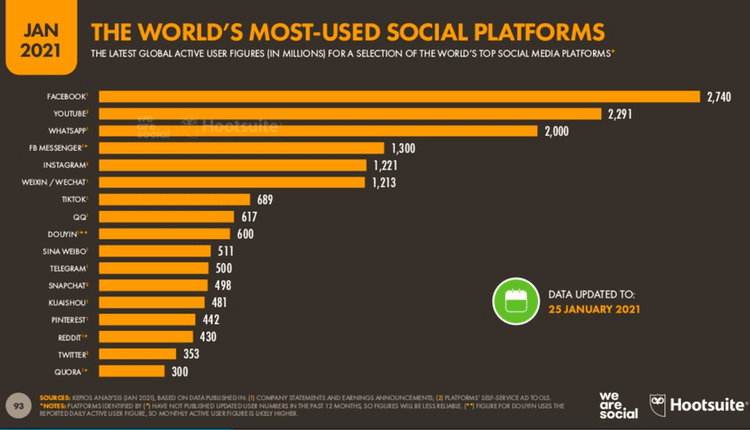
\includegraphics[width=\textwidth]{datos1.png}
    \caption{Plataformas sociales más empleadas}
    \label{datos1}
\end{figure}

A pesar de la polémica en torno a su seguridad, Zuckerberg aún reúne a la mayor parte de las redes sociales con más usuarios del mundo: WhatsApp (2.000 millones de usuarios), Messenger (1.300 millones de usuarios) e Instagram (1.221 millones de usuarios), que se conglomeran en el top 4 de este ranking, solo superados por YouTube.

El primer dato que salta a la vista es el impulso que la pandemia le ha dado a Instagram que pasó del sexto puesto en 2020 (1.000 millones de usuarios), al cuarto lugar en 2021 con un total de 1.220 millones de usuarios (+22\%). Sin embargo esto también se debe a que WeChat, la plataforma de mensajería instantánea más popular de China que ocupaba la quinta posición, ha mostrado solo un leve crecimiento y pasó de 1.151 millones de usuarios en 2020 a 1.213 este 2020.

\subsection{Impulso de TikTok}

Otro dato relevante es el increíble crecimiento de TikTok en este informe. Y es que si bien en 2020 este informe contabilizaba juntas a TikTok y Douyin, su filial en China con 800 millones de usuarios, este 2021 TikTok por sí sola, la red social ya cuenta con 689 millones de usuarios en el mundo. Y a pesar de mostrar un crecimiento moderado, entre las redes sociales con más usuarios del mundo continúan apareciendo las potentes plataformas chinas que en occidente son poco conocidas, como QQ o Baidu de las que te hemos hablado en su momento: redes sociales que salen de lo habitual en el día a día pero que son muy importantes para millones de personas en el planeta. Y mientras Twitter sigue cayendo entre las redes sociales más utilizadas en el mundo, del lugar número 13 al 16 y con 353 millones de usuarios este 2021 (+3,8\%), Pinterest continúa subiendo en el ranking y alcanza los 442 millones de usuarios (+37,2\%).

\subsection{Más de la mitad de la poblacion del mundo utiliza las redes sociales}

La pandemia impulsó el uso de redes sociales hasta lograr romper el hito de su historia: este 2021 el informe muestra que la penetración de las redes sociales ha superado por primera vez a la mitad de la población, con un total del 53.6\% de las personas en el mundo, es decir 4.200 millones.

\begin{figure}[ht!]
    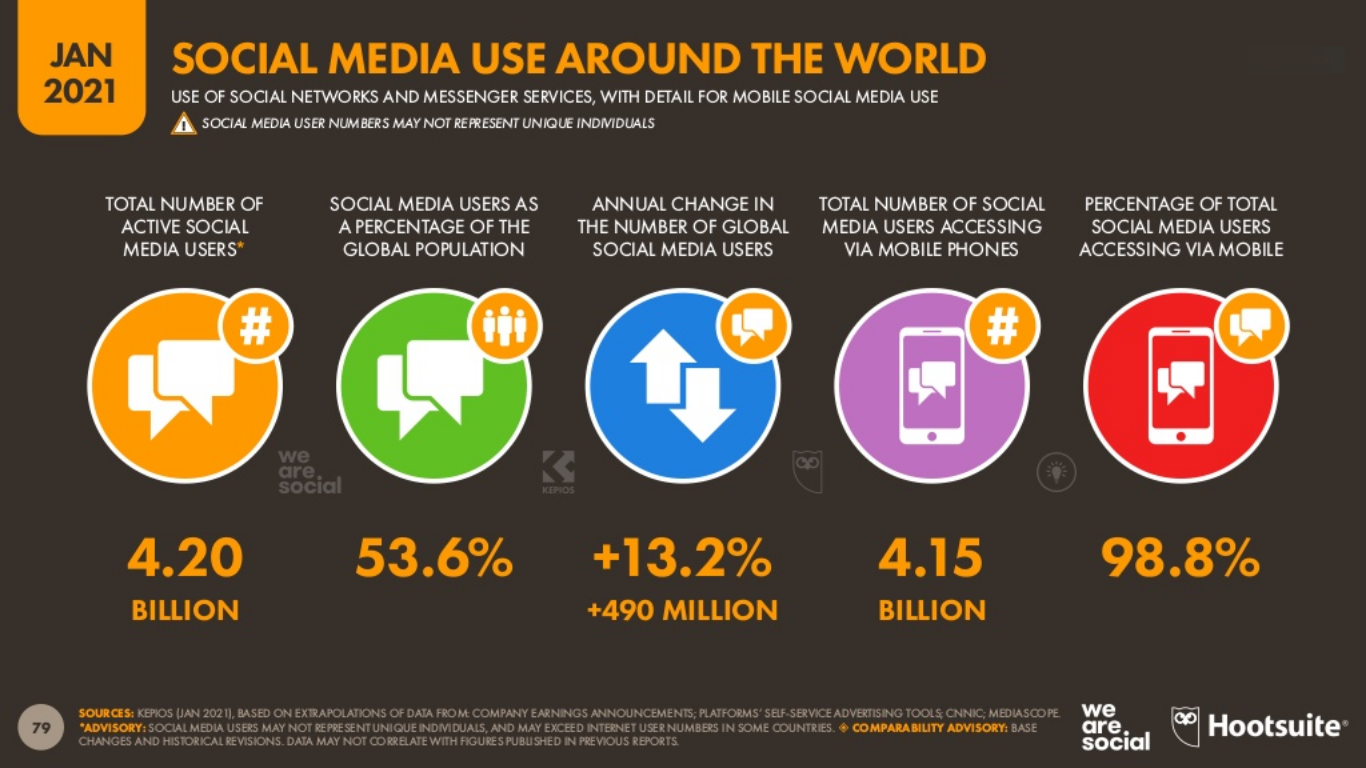
\includegraphics[width=\textwidth]{datos2.png}
    \caption{Uso de redes sociales a nivel mundial}
    \label{datos2}
\end{figure}

Esta cifra representa un crecimiento interanual del 13,2\% respecto al año anterior. Mientras el confinamiento se ha extendido a todo lo largo y ancho del planeta, muchos usuarios han optado por utilizar sus ordenadores de escritorio para realizar su trabajo o estudio a distancia, por lo que el porcentaje de usuarios móviles descendió levemente del 99\% a un 98,8\% este 2021.

Como es sabido, existen países en el que prácticamente el total de su población utiliza redes sociales, mientras en algunos otros este crecimiento es mucho más lento. Este 2021 los Emiratos Árabes Unidos continúan con su liderazgo en porcentaje de usuarios de redes sociales respecto a su población total, con un 99\%, seguido de cerca por Corea del Sur que sube una posición este año con 89.3\% de su población conectada a redes sociales. Taiwán cae al tercer lugar con un 88.1\%. Holanda (88\%) y Malasia (86\%) cierran el top 5. En cuanto a España ha subido rápidamente del lugar número 30 en 2020 al 14 con un 80\% de sus usuarios conectados al menos a una red social este 2021.

\begin{figure}[ht!]
    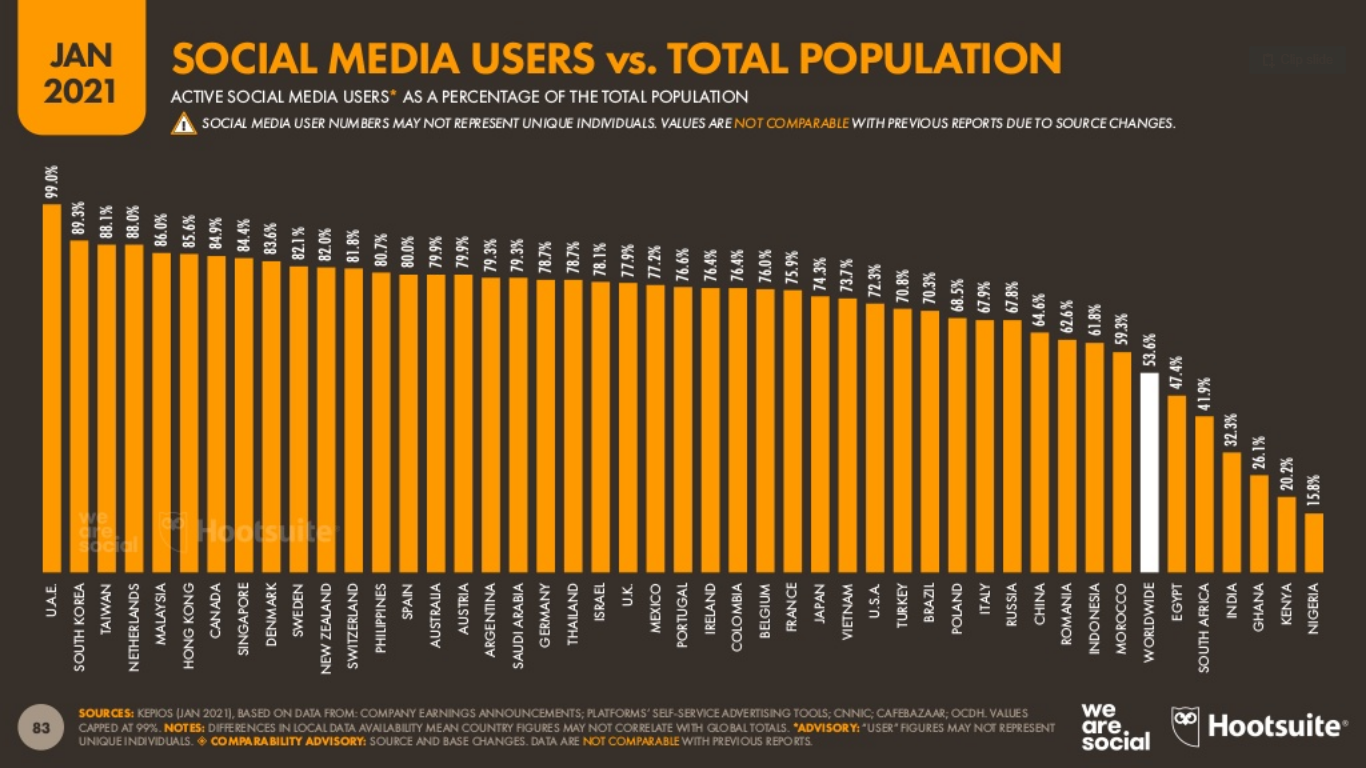
\includegraphics[width=\textwidth]{datos3.png}
    \caption{Usuarios de redes sociales}
    \label{datos3}
\end{figure}

\subsection{Tiempo de uso}

El tiempo promedio de uso de redes sociales por día a nivel global es de 2 horas con 25 minutos, sin embargo algunos países pasan más horas conectados a sus redes sociales que otros. Filipinas es el país en el que los usuarios pasan más horas revisando sus redes sociales, con 4 horas y 15 minutos en promedio, seguido por Colombia (3 horas y 45 minutos), Brasil (03:42), Kenia (03:42) y Nigeria (03:41). España se encuentra en el puesto número 33 de este ranking con un promedio de uso diario de redes sociales de 1:54 horas.

\begin{figure}[ht!]
    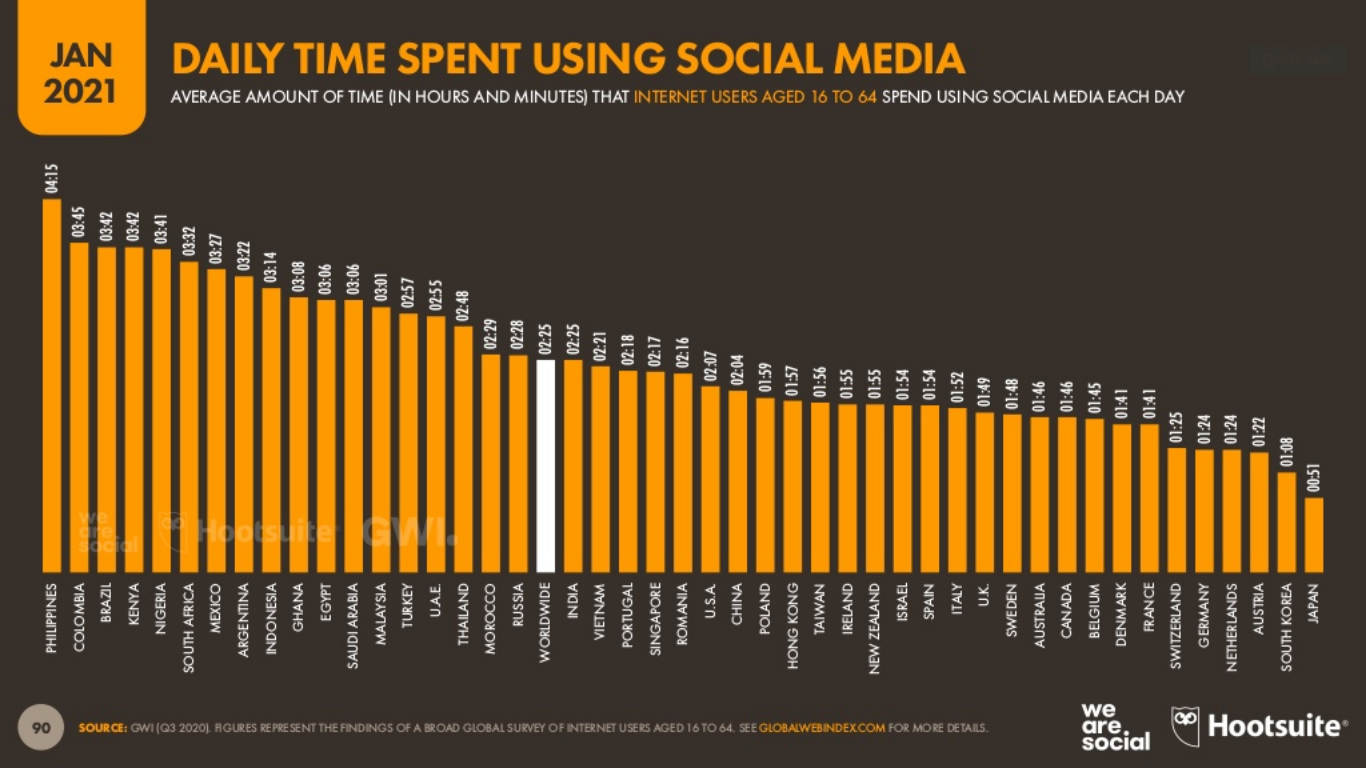
\includegraphics[width=\textwidth]{datos4.png}
    \caption{XXX}
    \label{datos4}
\end{figure}

El tiempo de uso diario de las redes sociales también diferencia la edad y sexo de los usuarios. Así, el mayor promedio de uso lo tienen las mujeres entre 16 y 24 años, con 3 horas y 14 minutos, seguidas por los hombres del mismo rango de edad, con un promedio de 2 horas y 39 minutos.

\begin{figure}[ht!]
    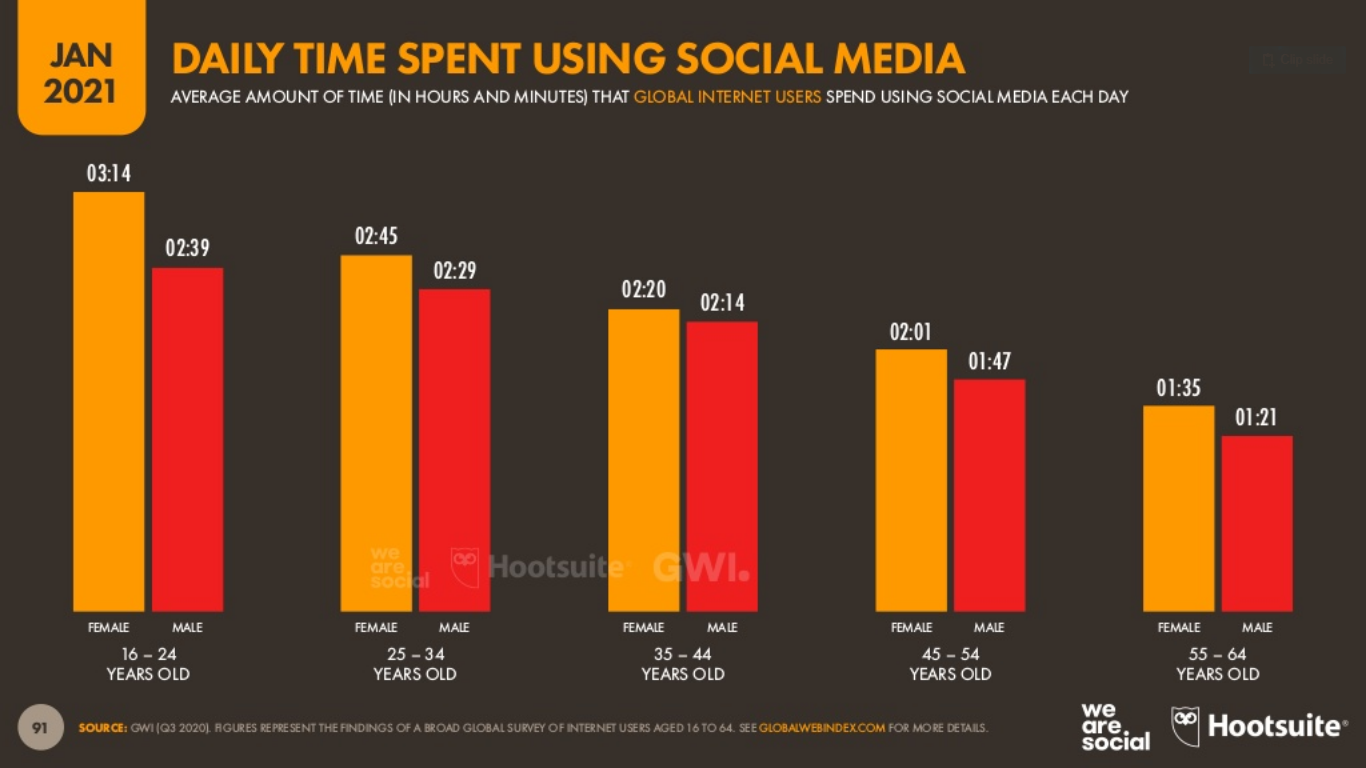
\includegraphics[width=\textwidth]{datos5.png}
    \caption{XXX}
    \label{datos5}
\end{figure}

En los últimos años, el tiempo de uso de las redes sociales se incrementó muy rápidamente hasta alcanzar un período de estabilidad. En 2015 los internautas pasaban un promedio de 1 hora con 51 minutos conectados a las redes sociales al día, que se incrementó a 2 horas con 15 minutos en 2017 que aumentó a 2 horas con 25 minutos en 2019 y se ha mantenido con ligeras variaciones desde entonces.

\begin{figure}[ht!]
    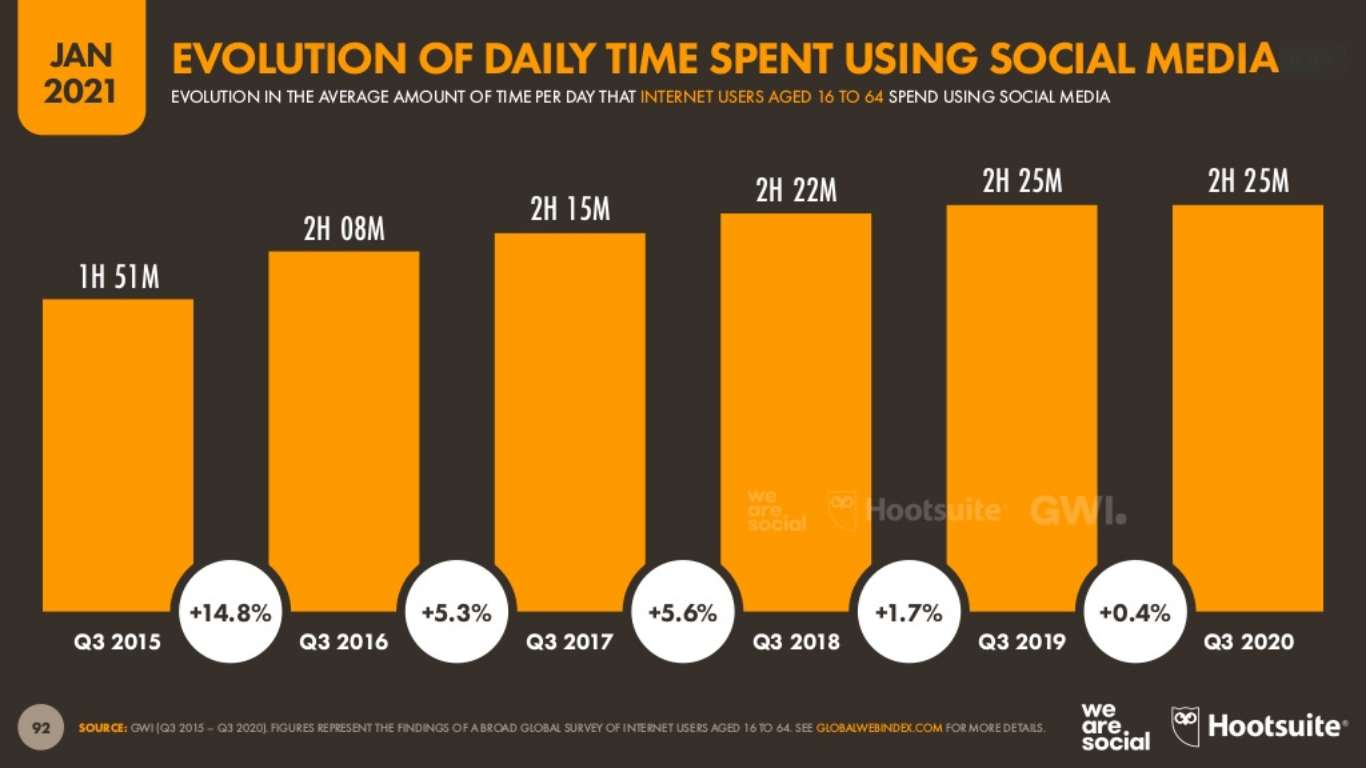
\includegraphics[width=\textwidth]{datos6.png}
    \caption{XXX}
    \label{datos6}
\end{figure}

Como dato adicional, el informe comparte esta tabla que compara a los usuarios de cada una de las redes sociales que también utiliza otra de ellas:

\begin{figure}[ht!]
    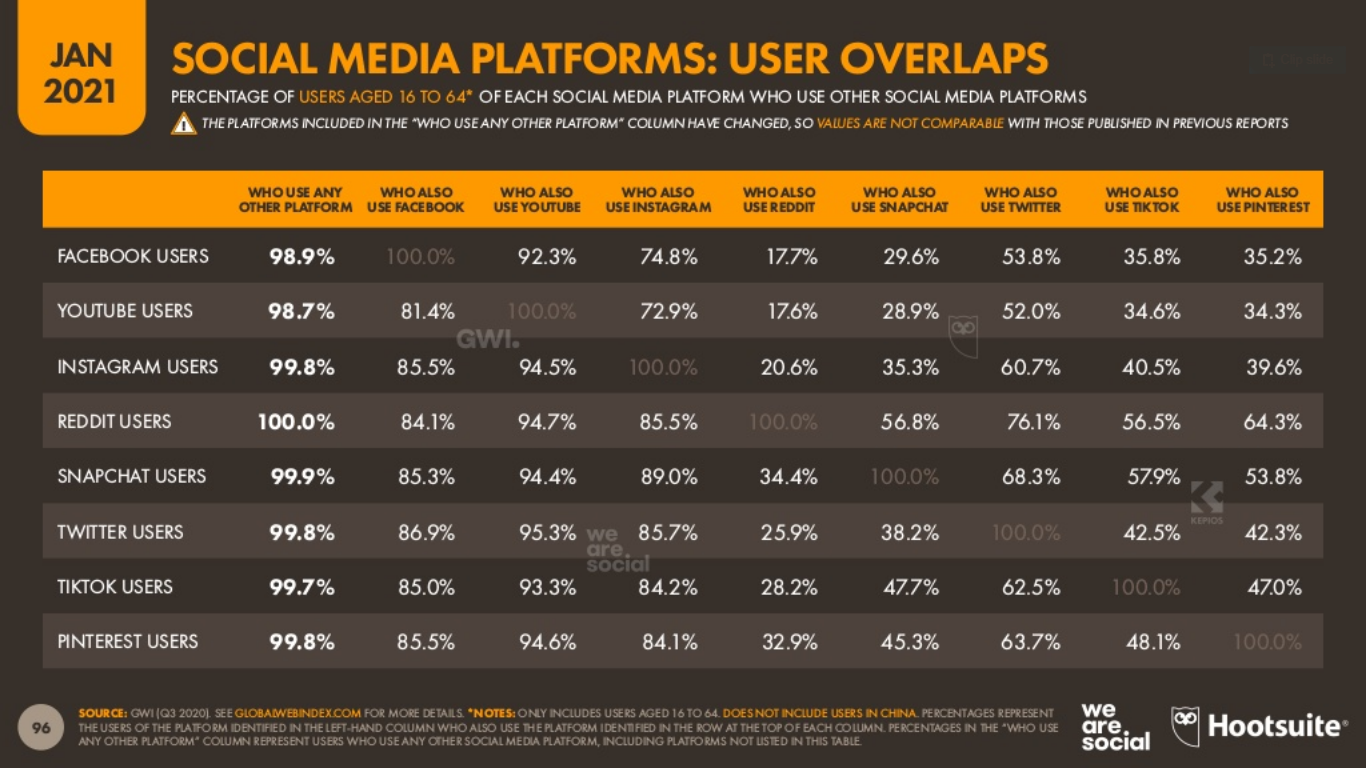
\includegraphics[width=\textwidth]{datos7.png}
    \caption{XXX}
    \label{datos7}
\end{figure}

\section{Problemas de redes sociales}

Las redes sociales se han convertido en un espacio en el que se forman y construyen relaciones, se configura la identidad, y permiten la expresión y el conocimiento del mundo. Sin embargo, las redes sociales también traen consigo algunos riesgos relevantes.

\subsection{Privacidad}

Son muchas las redes sociales que se pueden utilizar en el día a día. Algunas de las más populares son Facebook, Twitter o Instagram. Sirven para estar en contacto con amigos y familiares, dar la opinión o simplemente subir imágenes y vídeos. El abanico de posibilidades existentes es realmente amplio. La cuestión es que muchas de estas redes sociales han tenido problemas que pueden afectar a la seguridad. Incluso son los propios usuarios quienes cometen errores comunes.
\begin{itemize}
    \item Autorizar el acceso a ciertas aplicaciones. Uno de los problemas de privacidad más presentes en las redes sociales es el hecho de autorizar el acceso a ciertas aplicaciones. Algunas plataformas permiten conectar otros programas que pueden servir en el día a día y ofrecer herramientas muy útiles. Sin embargo en muchos casos se va a tener que autorizar el acceso a ciertas aplicaciones. Esto es un problema importante porque se está dando permisos a que recopilen información personal y puedan utilizarla en contra del usuario. Por tanto, es necesario tener cuidado siempre de qué aplicaciones se están empleando y a qué servicios se les está dando acceso.
    \item Compartir demasiada información personal. Por supuesto otro problema importante para la privacidad en redes sociales es compartir demasiada información. ¿Qué significa esto? Normalmente las plataformas pueden permitir que se ponga datos personales como el e-mail, nombre, lugar de trabajo o incluso el número de teléfono. ¿Realmente se quiere mostrar tantos datos? Un error común es hacer públicos más datos de los que realmente gustaría. En términos generales, no se necesita exponer tanta información personal para utilizar este tipo de servicios online.
    \item Caer en trampas y ataques cibernéticos. No hay que olvidarse de los ataques cibernéticos que pueden poner en riesgo la seguridad. En este caso, pueden ser por ejemplo ataques Phishing que buscan la manera de robar claves e información personal. Esto a fin de cuentas es un problema importante que puede poner en riesgo la privacidad. Para evitar esto lo mejor es tener sentido común y no caer en errores que pueden comprometer. También es vital contar con herramientas de seguridad, así como mantener los sistemas actualizados para corregir posibles vulnerabilidades que haya presentes.
    \item Cambios en los permisos de privacidad. Hay que tener mucho ojo con los posibles cambios en los permisos de privacidad. A veces esto puede cambiar y poner en riesgo las redes sociales. Especialmente hay que observar los complementos que se tienen instalados. No es extraño que una extensión cambie radicalmente en un momento dado y así lo haga su política de privacidad. En este sentido, es conveniente saber siempre qué tipo de complementos hay agregados en las redes sociales y qué permisos tienen. Esto es algo que puede verse en plataformas como Facebook, Instagram o Twitter.
\end{itemize}    

\subsection{Libertad de expresion}

Cada vez que se habla, se está asumiendo una determinada responsabilidad respecto a lo que se dice. Por ello, las palabras pueden provocar que otros hablantes acusen de haber sido imprudentes, de equivocarse e, incluso, pueden acarrear problemas legales si, por ejemplo, alguien considera que se ha violado su derecho al honor y a la privacidad.

Las redes sociales generan una sensación de anonimato y de desinhibición que favorece la proliferación de actos de agresión verbal, al mismo tiempo que muchos usuarios no son plenamente conscientes del gran alcance que pueden tener sus palabras en este medio. Por ello, las redes sociales se han convertido en un nuevo escenario para delitos como la difamación, el discurso de odio y el enaltecimiento del terrorismo.

No obstante, en los últimos años se está evidenciando la enorme dificultad que supone tratar de acotar los límites entre el derecho al honor y la libertad de expresión y ello ha avivado encontrados debates sociales en torno a cuál de estos dos derechos debe prevalecer. Todo ello parece aún más complicado en el entorno de las redes sociales, por las complejas dinámicas discursivas que en ellas se producen.

Pese a todo, la difamación, el discurso de odio y otros delitos similares no constituyen una de las áreas preferenciales de la lingüística forense, lo cual ha impedido el desarrollo de un aparato teórico-metodológico que permita analizar de manera sistemática textos que potencialmente vulneran el derecho al honor de un individuo o un grupo social determinado.

\subsection{Derecho al olvido}

La Ley Orgánica 3/2018, de Protección de Datos, regula el alcance de la protección de los datos en redes sociales, incluidos los derechos de acceso, rectificación, supresión, limitación del tratamiento, portabilidad y oposición. Los antiguos derechos “ARCO” se han visto ampliados por la normativa modificada, regulando nuevos derechos del titular. En particular, en el ámbito de las redes sociales, se han introducido novedades en lo referente al derecho al olvido o a la limitación del tratamiento de datos.

Uno de los problemas más habituales en la red es la dificultad a la hora de dar de baja un perfil o unos datos personales, para evitar que, en el futuro, otras personas puedan rastrear nuestra actividad. A los efectos de tutelar tal derecho y en garantía del efectivo respeto a tal derecho, han de tenerse  en cuenta las siguientes consideraciones respecto de cada uno de los casos:
\begin{itemize}
    \item El proveedor de servicios de Internet está obligado a eliminar el perfil de redes sociales de una persona si ésta lo solicita, sin más exigencias, ni requisitos.
    \item En el caso de los menores de edad, se refuerza tal derecho, no exigiendo la concurrencia de circunstancias especiales.
    \item Cualquier persona tiene el derecho a la eliminación de sus datos personales en redes sociales por falta de veracidad, o bien por desaparición de la razón que motivó la recogida.
\end{itemize}

Otra cuestión habitualmente problemática en las redes sociales es la gestión de perfiles de personas fallecidas. La nueva legislación facilita y agiliza la tramitación de la baja de tales perfiles a cargo de los herederos. Un instrumento especialmente útil a tal efecto es el “testamento digital”, pues permite a la persona dejar instrucciones en vida relativas a la gestión de sus datos en redes sociales tras la fecha de su fallecimiento; de tal forma que sus herederos podrán dirigirse a los prestadores de servicios de la sociedad de la información, al objeto de acceder a dichos contenidos, así como impartirles las instrucciones que estimen oportunas sobre su utilización, destino o eliminación.

\subsection{Fake news}

Las fake news o noticias falsas son bulos con apariencia de contenido periodístico que se difunden a través de portales de noticias y, sobre todo, de redes sociales. Suponen un problema porque muchos usuarios creen que su contenido es verídico y, por eso, estas fake news tienen la capacidad de alterar la opinión sobre temas políticos, sociales o la imagen pública de una marca o personaje.

Según un estudio de \href{https://www.simplelogica.com/es/}{Simple Lógica} y la Universidad Complutense de Madrid, el 86\% de los españoles confunden las fakes news con noticias reales. Y eso que el 60\% de los encuestados cree que sabe detectar una noticia falsa cuando la lee, pero el informe señala que solo el 14\% aciertan. Un rasgo común de las fake news son sus titulares alarmistas o irreales. Los fakes news son cada vez más frecuentes, pero sobre todo son rápidas. La investigación llevada a cabo en 2018 por el Media Lab del MIT (el prestigioso Massachusetts Institute of Technology) señalaba que las noticias falsas se difunden más rápido, más lejos y llegan a más personas que las informaciones verdaderas. 

Para combatir las fake news, se publican decálogos de buenas prácticas, surgen portales y herramientas de fact-checking, como \href{https://www.newtral.es}{Newtral} o Maldita (una práctica, por ejemplo, muy extendida en las entrevistas a líderes políticos) y se organizan foros y actividades para concienciar a la población. También se intenta atajar el problema desde la fuente. Las principales plataformas de distribución de las fakes news buscan mecanismos para detectar qué contenidos son falsos y así evitar su difusión. Por ejemplo, Facebook cuenta con un programa de verificación que, cuando considera que una es historia falsa, limita su visibilidad. Y en las búsquedas de YouTube se priorizan los vídeos que pertenecen a fuentes fiables de los que no lo son. Pero no es suficiente, de acuerdo con las autoridades que persiguen este tipo de prácticas.

Una de las razones de la revolución social que ha supuesto Internet es la posibilidad de que cualquier persona pueda publicar un contenido y compartirlo con otras personas. Del autor depende de que la información sea veraz, esté contrastada y no perjudique de manera intencionada. Por eso, los manuales de ética periodística, como este realizado por el Centro Internacional para Periodistas en colaboración con la UNESCO y el gobierno de Suecia –Ética Periodística en la Era Digital-, son otra buena herramienta para combatir las fake news.

\subsection{Deep fakes}

Hoy en día, en plena era de la información y las comunicaciones, somos testigos de un enorme avance en los métodos de desinformar y engañar a los usuarios. Comenzó como una broma, una forma de editar vídeos y poner nuestro rostro en famosos, pero la tecnología deepfake fue evolucionando hasta convertirse en una de las formas de fraude y desinformación más difíciles de reconocer a día de hoy.

\begin{figure}[ht!]
    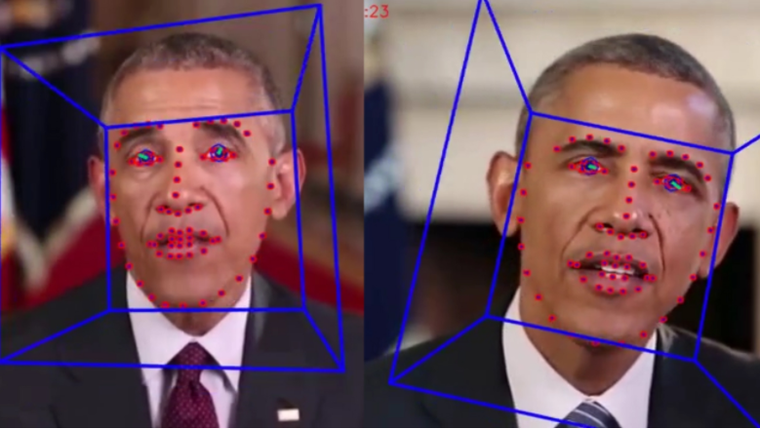
\includegraphics[width=\textwidth]{obama.png}
    \caption{XXX}
    \label{obama}
\end{figure}

La palabra \textbf{deepfake} es un término combinado de deep learning y fake, es decir:
\begin{itemize}
    \item \href{https://www.xataka.com/robotica-e-ia/deep-learning-que-es-y-por-que-va-a-ser-una-tecnologia-clave-en-el-futuro-de-la-inteligencia-artificial}{Deep learning} o aprendizaje profundo hace referencia a una de las ramas de la inteligencia artificial.
    \item Fake o falso, hace referencia a la elaboración de falacias en la red, del mismo modo que las fake news.
\end{itemize}

Se puede definir de manera sencilla los deepfakes como vídeos manipulados para hacer creer a los usuarios que los ven que una determinada persona, tanto si es anónima como si es personaje público, realiza declaraciones o acciones que nunca ocurrieron. Para la creación de dichos vídeos, se utilizan herramientas o programas dotados de tecnología de inteligencia artificial que permiten el intercambio de rostros en imágenes y la modificación de la voz.

Según lo anterior, podemos identificar dos tipos de deepfakes:
\begin{itemize}
    \item \textbf{Deepface}. En este caso, se trata de superponer el rostro de una persona en la de otra y falsificar sus gestos. En algunos casos, el resultado es tan realista que resulta muy difícil identificar el engaño o fraude.
    \item \textbf{Deepvoice}. En este otro caso se trataría de unir frases y palabras sueltas utilizadas por una persona para crear un discurso. Incluso, es capaz de clonar la voz original a partir de estos fragmentos.
\end{itemize}

El mayor peligro reside en la facilidad para crear este tipo de fraudes, y es que con una aplicación cualquier persona puede crear un vídeo falso pero muy creíble. Si ya es difícil detener la viralización de noticias falsas por la red, imaginemos si se trata de un formato en vídeo con la rapidez que tienen para extenderse por todo Internet.

Por otro lado, al ritmo al que avanza esta tecnología, en poco tiempo será casi imposible identificar si se trata de una falsificación o no, llegando a crear verdaderos estragos en la credibilidad o reputación de una persona. Si las noticias falsas ya influyen en temas tan importantes como en la crisis sanitaria que estamos viviendo actualmente debido al coronavirus, imaginemos lo que podría conseguirse con las deepfakes.

\section{Caso de estudio. Cambridge Analytica}

Cambridge Analytica es el nombre de una consultora británica que fue conocida mundialmente en 2018 después de ser la clave en uno de los escándalos de privacidad más grandes para las redes sociales y acceder ilegalmente a los datos de unos 87 millones de usuarios de Facebook en el mundo. 

\begin{figure}[ht!]
    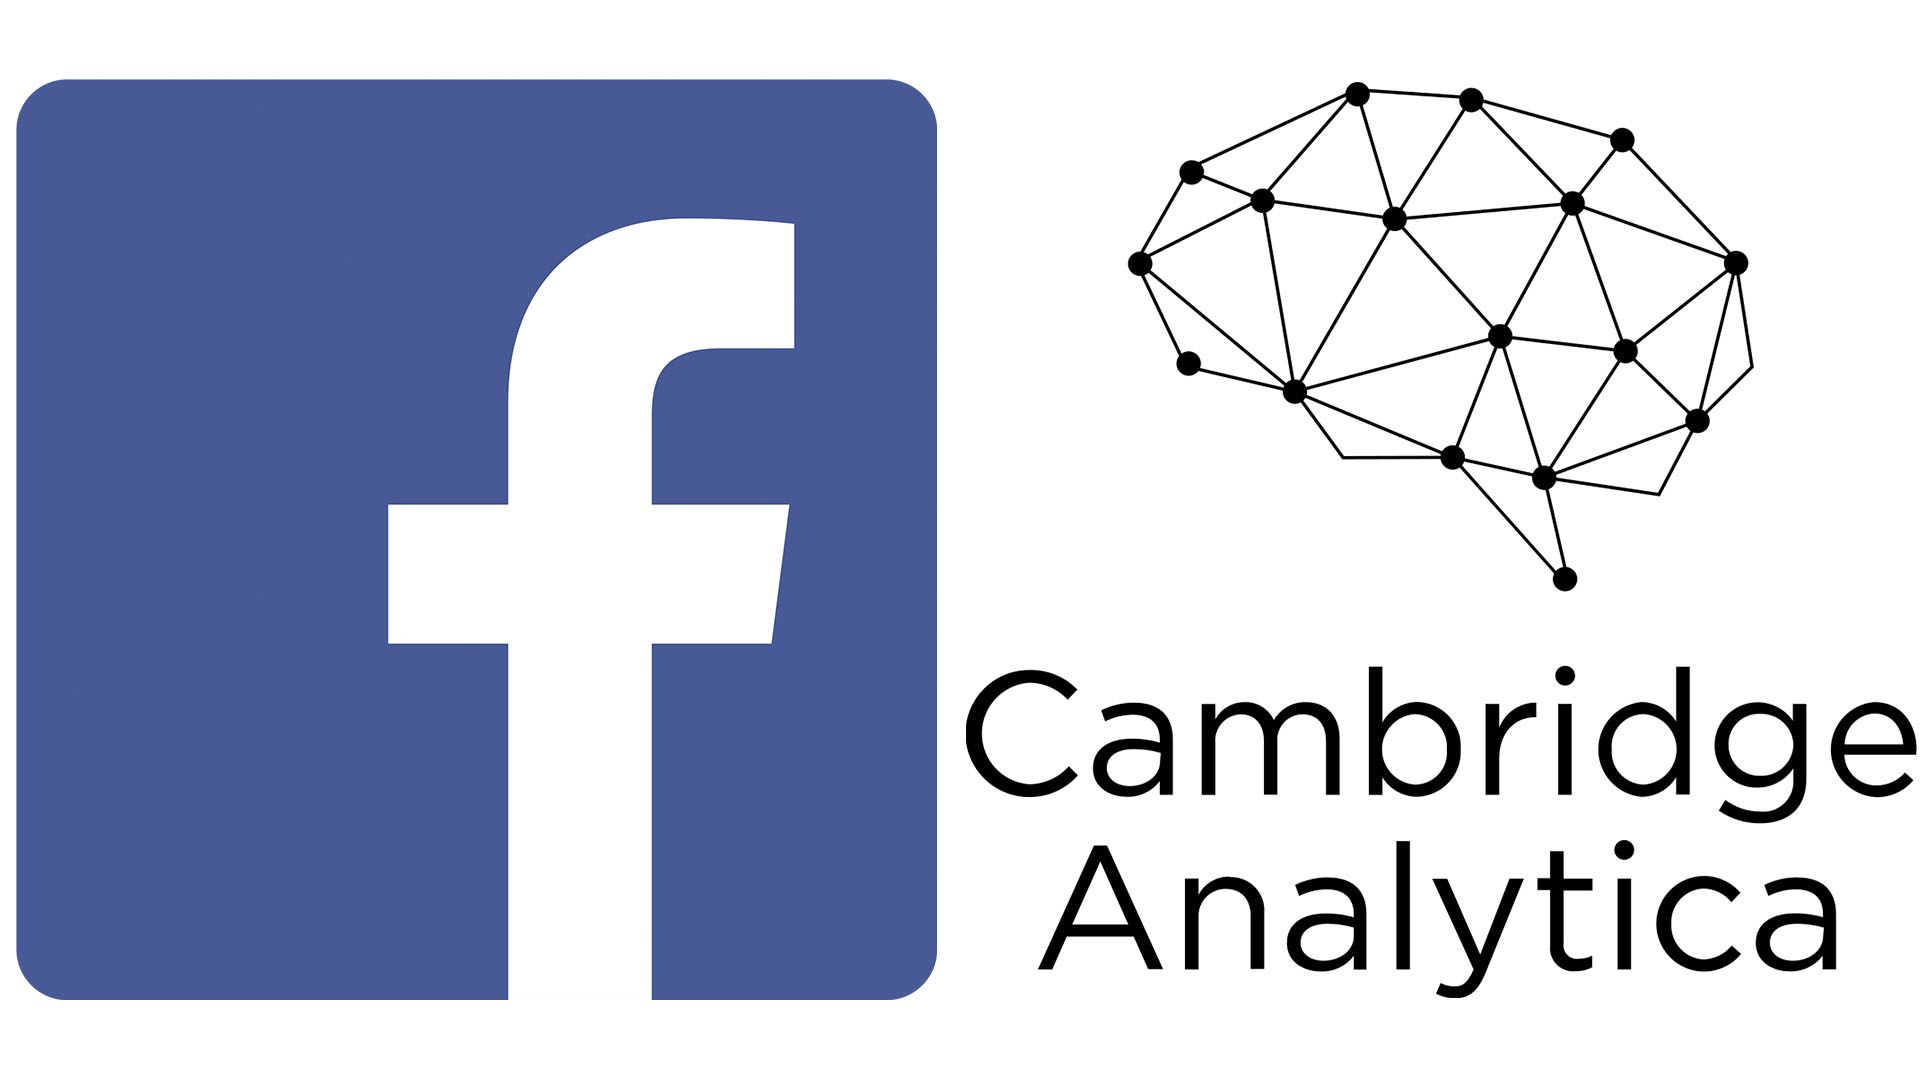
\includegraphics[width=\textwidth]{images/analytica.jpg}
    \caption{XXX}
    \label{analytic}
\end{figure}

Se trata de una firma de consultoría que fue fundada en 2013 (como parte del grupo SCL Group) y que se disolvió en mayo de 2018, meses después de que se conoció públicamente el escándalo de privacidad. La empresa, que tenía sede en Londres era experta en analizar datos y desarrollar campañas de comunicación y mercadeo con una metodología basada en 'puntos de comportamiento', que les permitía conocer rasgos de personalidad y "entender qué les importa a las personas, por qué se comportan como lo hacen y qué es lo que realmente impulsa su toma de decisiones", como rezaba en su sitio web.

La compañía no solo tenía clientes empresariales sino también grupos políticos. En su página listaban contratos con "más de 100 campañas", con clientes en América Latina y otras partes del mundo. Entre sus clientes, se encontraban la campaña presidencial de Donald Trump en 2016 y la campaña Leave.EU, uno de los grupos más grandes de Reino Unido a favor del Brexit.

Aunque su área de trabajo es la misma que podría tener una compañía de marketing digital, Cambridge Analytica tenía un enfoque en el uso de la tecnología, específicamente de ciencia de datos, mucho más avanzada, además de algunos postulados éticamente polémicos.  Por un lado, desde su fundación, la firma contó con una inversión de 15 millones de dólares por parte de dos estadounidenses: el republicano Robert Mercer y Steve Bannon, exjefe de estrategia de la Casa Blanca.

Aunque la consultora no estaba vinculada con la prestigiosa Universidad de Cambridge, si se benefició de su reputación y contrató a algunos investigadores de la institución académica. A diferencia de otras agencias, Cambridge Analytica comunicaba que poseía más de 5.000 puntos de contacto de más de 220 millones de estadounidenses con 100 variables de datos para modelar las audiencias y "predecir el comportamiento de personas con pensamientos similares".

\subsection{Origen del escandalo}

En marzo de 2018, algunos de los principales diarios de Reino Unido y EE. UU. (The Guardian y The New York Times) publicaron denuncias sobre millones de datos recopilados para enviar campañas de información a los votantes, vinculando a la consultora británica y a Facebook en el rumbo de las votaciones tanto de Donald Trump, como en la aceptación del Brexit.

Poco a poco surgieron las primeras explicaciones. Por un lado, el presidente ejecutivo, Alexander Nix, fue retirado de la firma que fundó. Por el otro, la presión mediática creció como una bola de nieve y entre las respuestas de funcionarios, ex empleados y consultores se conoció que todo empezó con un test de personalidad diseñado en 2013 por el investigador Aleksandr Kogan. Dicho test, llamado 'This is your digital life' (o esta es tu vida digital) fue llenado por cerca de 270.000 personas en Facebook. El test, favorecido por la plataforma, solicitaba permisos de acceso a nombre, correo, publicaciones en el muro, y otra información personal, incluyendo acceso a la red de 'amigos'. 

Kohan, profesor de la Universidad de Cambridge, desarrolló el test como un proyecto personal y luego lo vendió a la consultora británica. Testimonios de ex trabajadores a diferentes medios internacionales han sido claves para entender el caso y sostienen que la venta de dichos resultados de más de 200.000 usuarios violaba las políticas de Facebook al transferir o vender datos recopilados que solo podían ser usados para propósitos expresos de la aplicación a la que fueron entregados. 
Esa información, unida a la naturaleza de la consultora y sus avanzados sistemas, permitió que el alcance de actividades como datos de perfil, actualizaciones de estado o me gusta a páginas por parte de decenas de millones de usuarios fuera analizada. 

\subsection{Violacion a la privacidad}

En primer lugar, porque si bien algunos usuarios realizaron el test de Kohan con un pago de entre 2 y 5 dólares para vincular su perfil, no está claro si estaban totalmente informados sobre cómo sería usada esa información. A eso se le suma las personas que sin un pago de por medio realizaron el test voluntariamente, confiando en las políticas de privacidad de la red social. Estos entregaron sus datos sin creer o sospechar que podrían ser usados para fines de análisis y mercadeo por fuera de la red social. También, gracias a los permisos de acceso desmesurados, no solo se afectó al usuario que voluntariamente hizo el test sino a su red de contactos. En algunos casos, la aplicación accedió hasta a conversaciones privadas dentro de la red social, exponiendo lo que 'amigos' hablaban entre sí. 

Por último, porque Kohan violó las normas de Facebook y vendió la información haciendo que los datos que voluntariamente entregaron los usuarios para alguien fueran accedidos por otros desconocidos, sin autorización expresa y sin conocimiento alguno de los fines de uso de dicha información. 

\subsection{Rol de Facebook}

Pues además de haber sido la herramienta que usó Kohan para su test, Facebook falló en varios puntos del escándalo. El periódico británico The Guardian informó que Facebook había tenido conocimiento de esa violación a sus políticas. Christopher Wylie, un experto en datos y ex empleado de la consultora, reveló en diferentes entrevistas que después de dejar su cargo en la empresa en 2014 le advirtió a la red social sobre el uso que la compañía británica le daba a los datos. 

El mismo Mark Zuckerberg, fundador de la red social, reconoció después haber conocido en 2015 que el investigador Kogan había compartido los datos con la empresa Cambridge Analytica y que la información vendida se trataba de datos de usuarios de Facebook. La falla fue que en ese tiempo ni se le comunicó a las autoridades ni a los usuarios víctimas.

Facebook optó por vetar la aplicación de Kogan y prohibir a Cambridge Analytica realizar anuncios en su plataforma. También le pidió tanto al investigador como a la consultora que certificaran que habían borrado todos los datos obtenidos indebidamente y según Zuckerberg así lo dijeron. En esas, Cambridge Analytica aseguró que ninguno de esos datos había sido utilizado en sus servicios de consultoría, ni en el proceso de acompañamiento a la campaña de Donald Trump. 

En ese entonces, Facebook estaba con problemas de reputación después de que se conocieran también los intentos de manipulación extranjera y los miles de dólares de publicidad que invirtieron páginas y perfiles de Rusia e Irán para "dividir" las opiniones e influir en los comicios electorales. 

Mientras que Facebook y Cambridge Analytica han culpado a Kogan por el uso indebido de datos, el investigador ha dicho que es un 'chivo expiatorio' en medio del escándalo y que no solo Alexander Nix, exdirector de la consultora, había recibido la información sino que la consultora SCL Group (el otro grupo al que pertenecía Cambridge Analytica) era muy cercana a Facebook. El investigador, trató de implicar a la Universidad de Cambridge aludiendo que su trabajo había sido revisado y aprobado, pero una carta de 2015, publicada por varios medios reveló el rechazo de unos proyectos de Kogan por insuficiencias de privacidad.
